
\documentclass[11pt]{article}
\usepackage{natbib}
\usepackage{amssymb}
\usepackage{common}
\usepackage{graphicx}
\graphicspath{ {../img/} }

\title{HW3: Translation}
\author{Alex Lin \\ alexanderlin01@college.harvard.edu \and Melissa Yu \\ melissayu@college.harvard.edu \and Team Name: \textsc{Pudge}}


\begin{document}

\maketitle{}
\section{Introduction}

With the increasing globalization of our world, translation has become more and more important.  Prior to 2014, many automatic translation systems were either based on linguistic rules or statistical models.  However, with the emergence of deep learning, neural machine translation systems with end-to-end capabilities now dominate the field.  

In this problem set, we examine two such models: 1) a baseline sequence-to-sequence model and 2) an attention-driven deep learning model.  Our overall objective is to create translation systems that can translate German sentences to English sentences.  For an out-of-sample German test set comprised of 800 sentences, we generate 100 of the most probable 3-gram English starting-sentence translations as determined by our models.         

\section{Problem Description}

Let $\mathcal{V}_X$ be the German vocabulary and $\mathcal{V}_Y$ be the English vocabulary.  Let each word in a vocabulary be represented by a one-hot encoded vector with length equal to the vocabulary.  Given a German sentence (i.e sequence of words) $\boldx = [x_1, x_2, \ldots, x_S]$ and an English partial translation $[y_1, y_2, \ldots, y_{t-1}]$, the objective of translation is to accurately predict the distribution of the next English word $$y_t \vert y_1, \ldots, y_{t-1}, x$$ for $t = 1, 2, \ldots, T$ where $T$ is the length of $y$.  Let $q$ be our model's predictive distribution.  Let $(\boldx^{(n)}, \boldy^{(n)})$ be a single pair of German-English sentences that mean the same thing in our training set, for $n = 1, 2, \ldots, N$.  In training a model, we wish to adjust the model's parameters to minimize the \emph{average loss}, as defined by
\begin{align*}
L = \frac{1}{N} \sum_{n=1}^N \frac{1}{T} \sum_{t=1}^{T^{(n)}} \left(\ln q(y^{(n)}_t \vert y_1^{(n)}, \ldots, y_{t-1}^{(n)}, x^{(n)}) \right) \cdot y^{(n)}_t
\end{align*}
where $\cdot$ denotes the inner dot product and $T^{(n)}$ denotes the length of $\boldy^{(n)}$.  The standard metric used for evaluation is called \emph{perplexity}, as defined by
\begin{align*}
PPL = \exp L
\end{align*}

\section{Model and Algorithms}

We trained the three different models specified in the instructions.  These included (1) a baseline sequence-to-sequence model and (2) an attention-drive sequence-to-sequence model.

\subsection{Baseline Sequence-to-Sequence}
The baseline sequence-to-sequence model is comprised of an encoder LSTM and a decoder LSTM.  The encoder reads an input sentence $\boldx$ with length $T_x$ into a fixed-length context vector $c$, as follows:
\begin{align*}
h_t &= f(x_t, h_{t-1}) \quad \forall t = 1, \ldots, T_x \\
c &= j(\{h_1, \ldots, h_{T_x}\})
\end{align*}  
where $h_t$ is the hidden state of the encoder with $h_0 = \bold{0}$, and $j$ is a function of the hidden states.  In this case, we simply let $j(\{h_1, \ldots, h_{T_x}\}) = h_{T_X}$ (i.e. the last hidden state).  Next, we let $s_0 = c$ be the first previous hidden state of the decoder.  The decoder follows the recursion:
\begin{align*}
s_t &= g(y_t, s_{t-1}) \quad \forall t = 1, \ldots, \tilde{t}
\end{align*}
where $y_t$ is the $t$-th word of the supplied \emph{partial} output sentence with length $\tilde{t}$.  To predict the probability distribution over the $(\tilde{t} + 1)$-th word in the output, we simply have
\begin{align*}
q(y_{\tilde{t} + 1} \vert y_1, \ldots, y_{\tilde t}, \boldx) = \text{softmax}(W s_t + b)
\end{align*}  
where $W$ is a $\lvert V_Y \rvert \times n_\text{hid}$ matrix and $b$ is an $n_\text{hid}$-dimensional vector.  Note that 
$$n_\text{hid} = \dim s_t = \dim h_t$$
is the number of hidden states in each of the two LSTMs.

\subsection{Sequence-to-Sequence with Attention}
Next, we incorporate attention into the baseline model. We once again experiment with vanilla and bidirectional LSTM's for both the encoder and decoder networks.

The encoder network consists of an embedding layer, $M^{(e)}\in\mathbb{R}^{m_e\times\lvert \mathcal{V}_s \rvert}$, followed by an $N^{(e)}$-layer LSTM with hidden size $H^{(e)}$. The encoder returns the hidden and cell states $(h_S, c_S)\in \mathbb{R}^{N^{(e)}\times H^{(e)}}$ for the last word in the input, along with the the outputs $o_s\in \mathbb{R}^{H^(e)}$ at the last LSTM layer for all words in the input.

The decoder network also consists of an embedding layer, $M^{(d)}\in\mathbb{R}^{m_d\times\lvert \mathcal{V}_t \rvert}$, followed by an $N^{(d)}$-layer LSTM with hidden size $H^{(d)}$. The LSTM hidden and cell states $(h_0, c_0)\in \mathbb{R}^{N^{(d)}\times H^{(d)}}$ are initialized using the last "forward" direction encoder hidden and cell states $(h_S, c_S)$. We let $o_t\in \mathbb{R}^{H^(d)}$ be the output of the LSTM. We compute the dot product attention over the inputs for each timestep $t$ by taking
\[
\alpha_t = \mathcal{S}(f(o_{1:S}, o_t)),
\]
where $f = (\boldW o_{1:S} + b)\cdot o_t$; the linear layer $(\boldW, b)$ over the encoder output is necessary to transform its hidden size to match that of the decoder. Using the attention weights, we construct a context vector $c_t$:
\[
c_t = \sum_{s=1}^S \alpha_{ts} o_s
\]
Then, the probability distribution over our target vocabulary words returned by the decoder is
\[
p(y_t\given y_{<t}, \boldx) =
\mathcal{S}(\boldW' [o_t, c_t]^\trans + b')
\]    


\section{Experiments}

We performed several experiments to tune the hyper-parameters of our models. The attention model seemed to perform the best. In-depth explanations of our tuning procedure and associated results can be found in this section. Note that all perplexities reported in table \ref{tab:results} are test set perplexities.

\begin{table}[H]
\centering
\begin{tabular}{llr rr}
 \toprule
 Model &  & Validation Perplexity & & Kaggle Score\\
 \midrule
 \textsc{Baseline Sequence-to-Sequence} & & 13.831 & &0.24806\\
 \textsc{Sequence-to-Sequence with Attention} & &7.55&&0.27141  \\
 \bottomrule 
\end{tabular}
\caption{\label{tab:results} Language perplexities and Kaggle scores of our models.}
\end{table}


\subsection{Baseline Sequence-to-Sequence} 
The main parameters that we tuned were (1) the embedding dimensions of the two vocabularies, (2) the number of hidden states $n_\text{hid}$, (3) the number of hidden layers in each LSTM, (4) the dropout rate, and (5) whether or not to reverse the input sentence $\boldx$.    

The model that obtained the best validation perplexity of 13.831 had embedding dimensions of 1000 each, $n_\text{hid} = 1000$, 2 hidden layers in each LSTM, a dropout rate of 0.2, and reversed input.  We used a stochastic gradient descent optimizer that ran for 16 epochs with an initial learning rate of 1 that was successively halved during the 7th and 14th epochs.  The batch size was 32 and the maximum norm of any gradient used during training was set as 5.

Here are our results from varying embedding dimensions (assume all other variables are as listed above).  We found that increasing the embedding dimensions too much led to overfitting (i.e. low train perplexity, but higher test perplexity).  

\begin{center}
	\begin{tabular}{ c | c c c c c}
		 \text{Embedding Dimension} & 100 & 200 & 500 & 1000 & 1500  \\
		\hline
		Val. Perplexity & 15.82 & 14.52 & 14.01 & 13.83 & 15.27
	\end{tabular}
\end{center}    

Here are our results from varying $n_\text{hid}$.  

\begin{center}
	\begin{tabular}{ c | c c c c c}
		 $n_\text{hid}$ & 100 & 200 & 500 & 1000 & 1500  \\
		\hline
		Val. Perplexity & 14.11 & 14.15 & 13.87 & 13.83 & 13.94
	\end{tabular}
\end{center}    

Here are our results from varying the number of hidden layers in the two LSTMs.  

\begin{center}
	\begin{tabular}{ c | c c c c c}
		 Number of Hidden Layers & 1 & 2 & 3 & 4   \\
		\hline
		Val. Perplexity & 18.81 & 13.87 & 14.66 & 14.67
	\end{tabular}
\end{center}    

Here are our results from varying the dropout rate. 

\begin{center}
	\begin{tabular}{ c | c c c c c}
		 Dropout Rate & 0.1 & 0.2 & 0.3 & 0.4   \\
		\hline
		Val. Perplexity & 14.08 & 13.87 & 13.92 & 13.91
	\end{tabular}
\end{center} 

And here are our results for deciding whether or not to reverse the input sentence $\boldx$.  
\begin{center}
	\begin{tabular}{ c | c c c c c}
		  & No Reverse & Yes Reverse   \\
		\hline
		Val. Perplexity & 13.99 & 13.87
	\end{tabular}
\end{center} 

To generate predictions for the Kaggle competition, we used beam search with a beam of 100.  Our Kaggle score obtained from the baseline sequence-to-sequence model trained with the most optimal parameters is 0.24806.   

\subsection{Sequence-to-Sequence with Attention} 
We train the attention model using full teacher forcing and additionally mask the source at words that are padded. We use the Adam optimizer with learning rate 0.001, decaying the rate by 0.5 each epoch after 8 epochs. The choice of optimizer was important, leading to a drop in validation perplexity from 12.83 to 7.55, all else held constant. All gradients are clipped to a maximum total norm of 10. We train for a maximum of 30 epochs, using the validation set perplexity as criteria for early stopping. 

We experimented with initializing the embeddings matrices with pretrained vectors (e.g., GloVe, fastText), but found that this did not give a significant performance improvement. Likewise, limiting the max norm for embedding values did not lead to performance gains.

Our final model uses single-direction 2-layer LSTM's with a hidden size of 200 for both the encoder and decoder and a dropout of 0.3 during training. This model achieves a training set perplexity of 8.67 and a validation set perplexity of 7.55. Surprisingly, bidirectional LSTM's performed poorly on this task, overfitting to the training target data.

Figure \ref{fig:attn} shows sample attention plots for our final model.

\begin{figure}[H]
	\begin{center}
		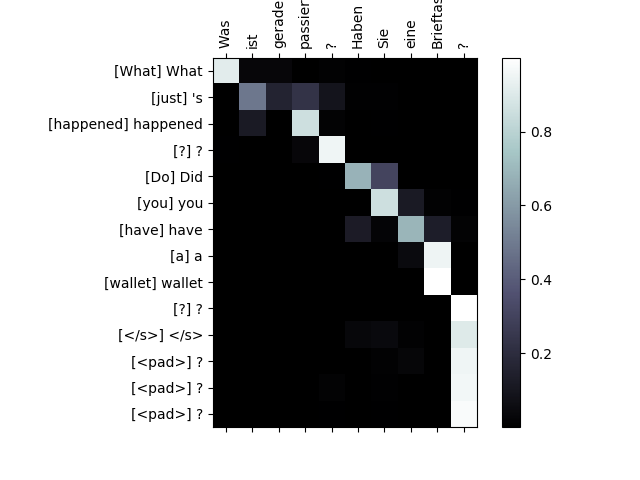
\includegraphics[scale=0.5]{attn_0}
		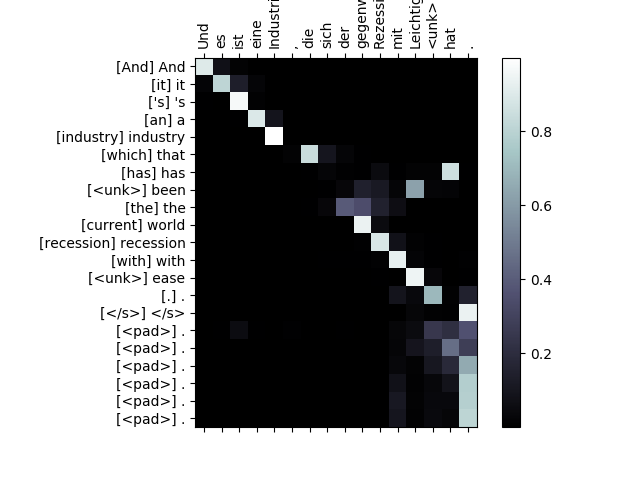
\includegraphics[scale=0.5]{attn_1}
		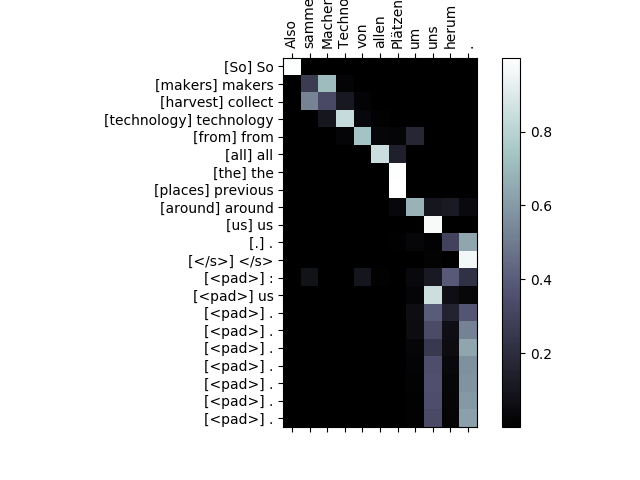
\includegraphics[scale=0.5]{attn_2}
		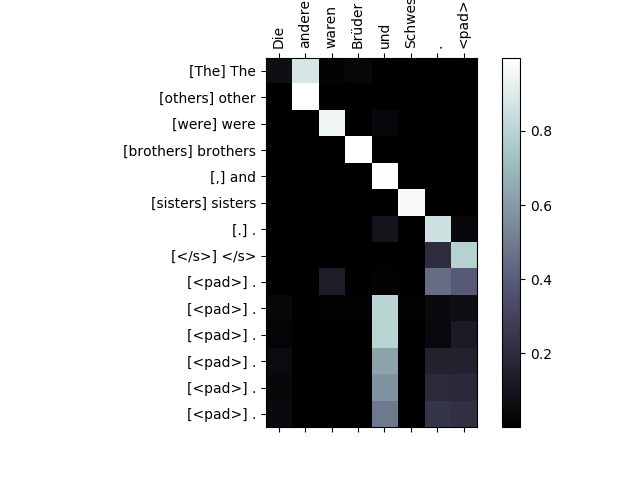
\includegraphics[scale=0.5]{attn_3}
		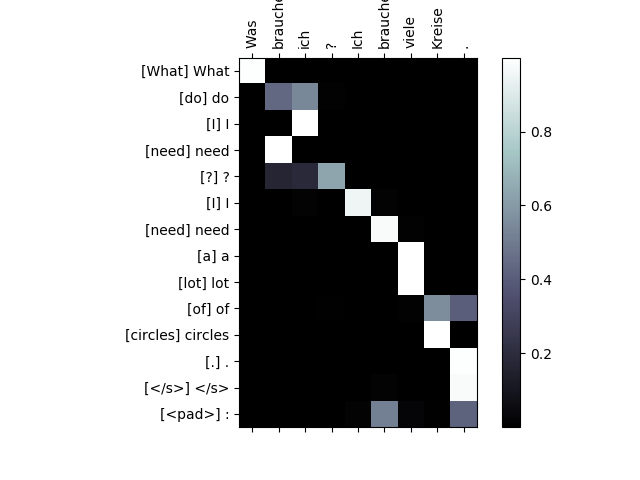
\includegraphics[scale=0.5]{attn_4}
		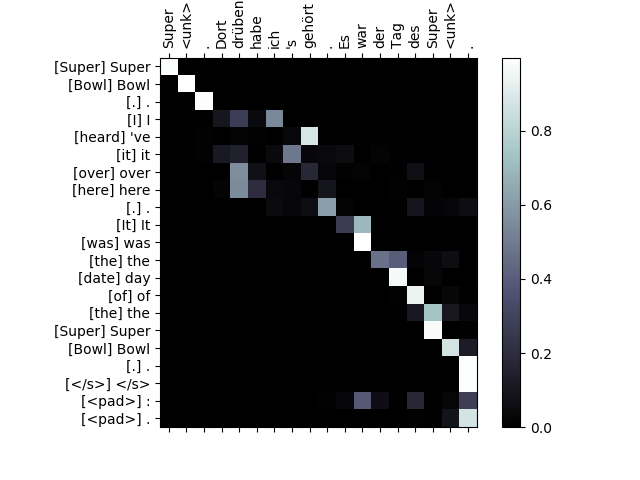
\includegraphics[scale=0.5]{attn_5}
		\label{fig:attn}
		\caption{Attention plots for a selection of sentences from the training dataset. The source (German) sentences are shown on the $x$ axis, and the targets are shown on the $y$ axis. The predicted target words are shown perpended with the true word in braces.}
	\end{center} 
\end{figure}


\section{Conclusion}
In this practical, we implemented two models to predict the most likely translations: A baseline LSTM sequence-to-sequence model and a version of this model with dot product attention. We also implemented a beam search algorithm to make predictions using our models. Our experiments on the German-English dataset show that the both the baseline model and the model with attention perform quite well, scoring well above the Kaggle baseline.


\bibliography{writeup}
\nocite{*}
\bibliographystyle{apalike}

\end{document}
